\documentclass[letterpaper]{article}
\usepackage[colorlinks]{hyperref}
\usepackage{aaai}
\usepackage{times}
\usepackage{helvet}
\usepackage{courier}
\usepackage{amsmath}
\usepackage{graphicx}
\frenchspacing
\setlength{\pdfpagewidth}{8.5in}
\setlength{\pdfpageheight}{11in}
\setcounter{secnumdepth}{0}

\title{Chinese Chess AI Agent}
\author{Suting Chen, Zeen Chi, Bingnan Li, Zhongxiao Cong, Yifan Qin\\
School of Information Science and Technology\\
ShanghaiTech University\\
No.393 Middle Huaxia Road\\
Shanghai, China 201210\\
\texttt{\{chenst,chize,libn,congzhx,qinyf1\}@shanghaitech.edu.cn}
}

\begin{document}

\maketitle

\begin{abstract}
\begin{quote}
Chinese Chess is one of the most classical problems for Artificial Intelligence.
In this project, we implement several AI agents to play Chinese Chess, utilizing Minimax Search, Reinforcement Learning, and Monte-Carlo Tree Search.
Based on the Chinese Chess application fully developed by our team, together with a random agent and a mouse/keyboard agent, we compare the performance of these three AI agents, including their superiority over the random one and their relative performance.
We also try to conduct competitions between the best AI agent with the real Chinese Chess AI on the Internet.
Our code is available at \url{https://github.com/caoster/CS181-Final-Project}.
\end{quote}
\end{abstract}


    \section{Introduction}\label{sec:introduction}

    \subsection{Motivation}\label{subsec:motivation}
    Chinese chess is a typical Combinatorial Game, which possesses properties of zero-sum, perfect information, deterministic, discrete and sequential.
    The property of perfect information means all possible moves are known to both players.
    Compared with other traditional Chinese games like Mahjong and Pai gow, this property significantly reduces the state space.
    Besides, given that Chinese chess has a series of rules and constrains, the number of possible moves is limited, which further reduces the state space.
    Take GO as a counterexample, for each step, the number of possible moves is 361, the size of state space is about $3^{361}\approx 10^{172}$ while it is about $10^{40}$ in Chinese chess.

    \subsection{Basic Framework}\label{subsec:framework}
    In this project, we utilized \emph{tkinter} and \emph{JUCE} to implement python and C++ version of Chinese Chess application(shown in Figure~\ref{fig:figure}).
    Given the complex rules of draw determination, we simplified the rule and set draw if none of the two players eats any piece in 40 steps.
    \begin{figure}
        \centering
        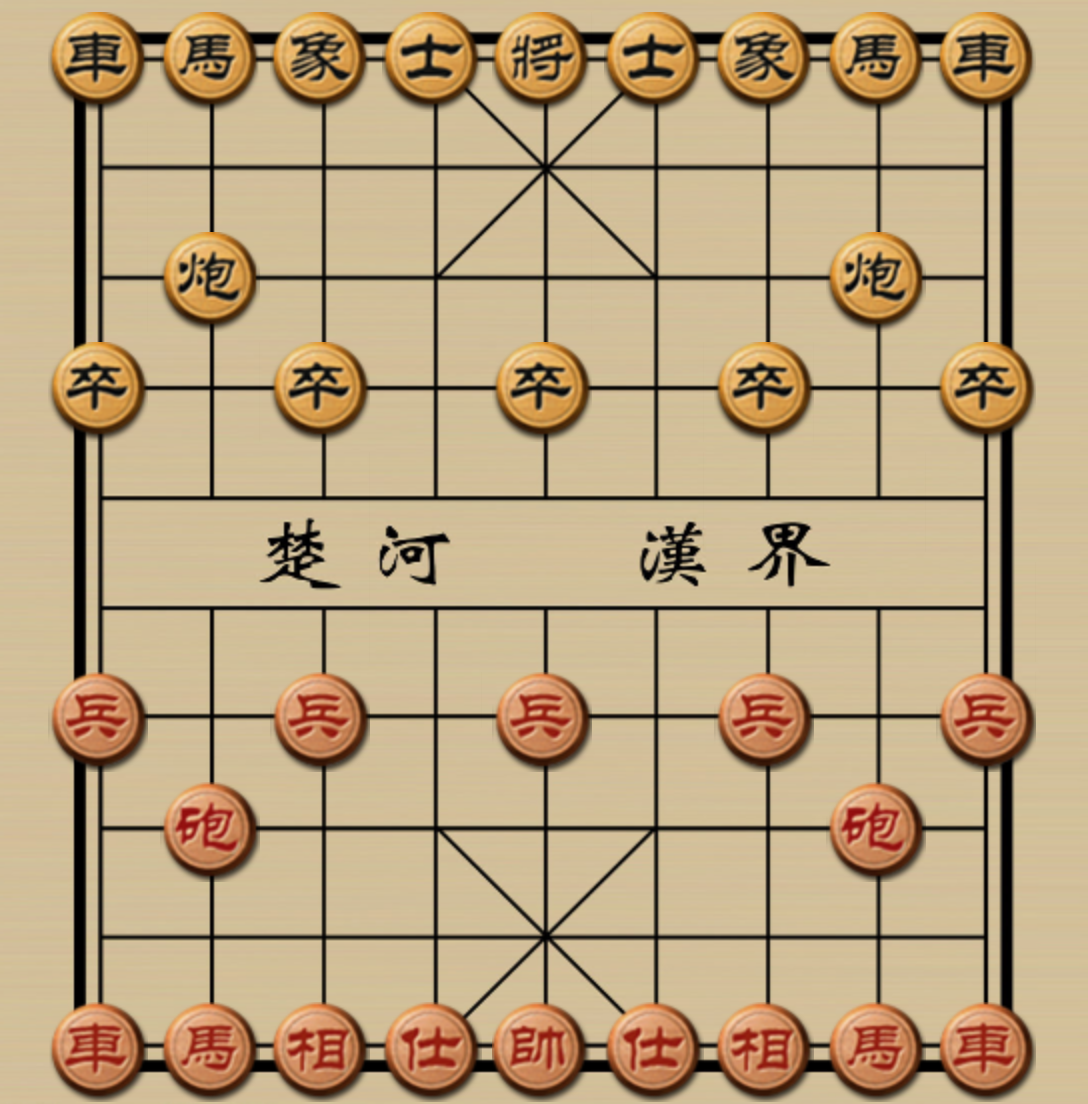
\includegraphics[width=0.4\textwidth]{img/overview}
        \caption{Overview of the Chinese Chess framework}\label{fig:figure}
    \end{figure}
    \section{Methods}\label{sec:methods}

In this section, we will introduce three methods we used in this project.
They are Minimax Search, Reinforcement Learning, and Monte-Carlo Tree Search, respectively.
We will briefly introduce their basic ideas and then explain how we implement them in our project.

\subsection{Minimax Search}\label{subsec:minimax-search}
The most straightforward method for the adversarial search based game is minimax search algorithm.
As taught in the class, the minimax search algorithm is a recursive algorithm that is used to find the optimal move for a player, assuming that the opponent also plays optimally.
\subsubsection*{Basic Idea}
The search tree is constructed based on the states and actions.
Each state is a tree node, while each action $a$ transit state $s$ to $s'$ is a tree edge.
The root of the tree is a max layer, and for the following layers, the nodes are alternately min and max layers.
The value of a node is the value of the state it represents.

However, it is impossible to build a full search tree for the chess board, because the complexity grows exponentially as we search deeper.
Therefore, we utilize depth-limited search strategy, which means the searching process terminates when the depth of the tree reaches a certain value, for example, 3.
Actually, as the game plays, there will be fewer pieces on the board and hence smaller branching factor, so we utilize iterative deepening based on the number of the pieces on the board.
As the pieces become less, we search deeper.

\subsubsection*{Evaluation Function} When searching process terminates, we have to evaluate the score of the state of the so-called leaf node.
Based on~\cite{yen2004computer}, we have considered the following factors when designing the evaluation function:
\begin{itemize}
    \item The power of each piece.
    We assign different values to different types of pieces, and the more powerful the piece is, the higher the value is.
    For example, we assign 600000 to General, 600 to Chariot, 450 to Cannon, 270 to Horse, etc.
    \item The position of each piece.
    We assign different values to different positions of the pieces, and the more advantageous the position is, the higher the value is.
    More specifically, we design a $10\times 9$ matrix (which is the size of the board) for each piece, with each value
    representing the advantage of the position.
    \item The flexibility of each piece.
    Based on the moving range, different types of pieces have different flexibilities.
    We first assign different fixed values to each type, and calculate how many positions can each piece reach.
    We multiply the fixed value to the calculated value, and the result is the flexibility of the piece.
    \item The value of threatening others.
    How many enemy pieces can be threatened by the current piece and the value of the threatened pieces really matter.
    We calculate the number of threatened pieces and the value of the threatened pieces, and the result is element-wise multiplication of the two values.
    \item The value of being threatened.
    We have to calculate how many piece can threaten the current piece.
    After the number is calculated, we can multiply it by the power of the piece.
    \item The value of being protected.
    It is also important to consider how many pieces can protect the current position, that is, if the current piece is killed by the enemy, how many allies can revenge for it.
    After the number is calculated, we can multiply it by the power of the piece.
\end{itemize}
For each leaf node state, we respectively calculate the weighted sum of the above factors of the player and the opponent, and the difference is the evaluation value of the state.

\subsubsection{Optimization}
We apply alpha-beta pruning method to the minimax search algorithm, which can reduce the number of nodes that need to be evaluated.
It stops evaluating a move when at least one possibility has been found that proves the move to be worse than a previously examined move.
Such moves need not be evaluated further.
When applied to a standard minimax tree, it returns the same move as minimax would, but prunes away branches that cannot possibly influence the final decision.

\subsection{Reinforcement Learning}\label{subsec:reinforcement-learning}
Since we need to know how to take each step, i.e., get the action, we use the Q-learning method.
\subsubsection{Q value}
The Q value is $Q_{k}(s,a)$
where s denotes the current state of the game and a denotes the current action.
We use the board to represent the current state of the game. Considering that the 
starting point and the landing point of this action will be different, we define the 
action as a tuple, which records which piece is picked and where this piece lands.
\subsubsection{Reward function}

\subsubsection{Training design}
Considering the training time, we train our Qlearning agent as a red side with Random agent on the black side. 
After Qlearning agent makes a move, we record the current state of the board and its 
actions, and from these two we calculate the reward that the Qlearning agent gets in this move 
as r1. Next, after the random agent makes its next move, we get the reward 
that the Random agent gets in this move as r2. Then, at the end of this round, the actual 
reward that Red gets is (r1-r2). So the sample estimate is
\begin{align*}
    sample=(r1-r2)+\gamma max_{a'}Q(s',a')
\end{align*}
Then we update the q-value of $Q(s,a)$
\begin{align*}
    Q(s,a)\leftarrow (1-\alpha)Q(s,a)+\alpha [sample]
\end{align*}
Since we need to explore as many different states as possible in the early stages of training, 
we introduced the $\epsilon$-greedy function. Setting epsilon to 0.5 gives our agent a 50 percent chance of 
picking the optimal policy based on $argmax_{a}Q(s,a)$ and a 50 percent chance of taking the policy randomly.

\subsubsection{Training}
Due to memory limitations, the training limit is 4000 epochs. The gamma is set to 0.8 and the 
learning rate is set to 0.8 for the first 1000 epochs, 0.5 for 1000 to 2000 epochs, 0.2 for 2000 
to 3000 epochs, and 0.1 for 3000 to 4000 epochs.
We write the explored qvalue to a txt file in the form of json. All values of the current Q(s,a) are 
recorded once every 100 epochs.

\subsection{Monte-Carlo Tree Search}
\label{subsec:monte-carlo-tree-search}
It is known that the search strategy that AlphaGo uses is the Monte Carlo Tree Search(MCTS). 
The MCTS search algorithm can effectively solve the problem when the state space is too big. 
Although Chinese Chess does not have the search space as big as the Go game, where players can have hundreds of choices to put their chesses at each step, players still have about fourty choices to move their pieces, which indicates a large search space. 
So we think that it may be feasible to use the MCTS search algorithm in the Chinese Chess. 
As MCTS was not fully introduced in the lectures, here the basic idea of MCTS will be introduced and our implementation of MCTS will also be talked about. 
\subsubsection{Basic Idea}
MCTS search algorithm build the search tree node by node according to the outcome of the simulation results. 
To be more specific, the search tree is built during the iteration of four steps, Selection, Expansion, Simulation and Backpropagation. 

In the Selection step, starting from the root node, the optimal leaf node will be chosen recursively until a leaf node $L$ is reached. 
In the Expansion step, if the leaf node $L$ that we reached is not the terminal node, we can have several child nodes of the leaf node. 
One of the child nodes of the leaf node $L$ will be expanded and added to the search tree. 
Then in the Simulation step, we will start a simulated game from the child node $C$ that we just expanded and get a final result. 
Finally in the Backpropagation step, we will back propagate the result from the child node to the root node of the search tree in order to update the movements or the choices sequence with the simulation result. 

If only the estimated values of the simulation result of the nodes are utilized, chances are that the node choice of the Selection step will concentrate within a few nodes. 
Other nodes or the movements may be less explored. 
In order to avoid the concentration, both the estimated value and the visit time of the node is used to find the optimal leaf node. 
There are several algorithms that can be used to calculate the best child of a node, such as the Upper Confidence Bound(UCB) algorithm. 

%%%%%%%
%https://www.cs.swarthmore.edu/~mitchell/classes/cs63/f20/reading/mcts.html
%https://zhuanlan.zhihu.com/p/26335999
%https://zhuanlan.zhihu.com/p/30458774
%%%%%%%
\subsubsection{Implementation}
In our implementation, the algorithm that is used to get the best child of a node is the Upper Confidence Bound for Tree(UCT) which is an application of UCB algorithm. 
The algorithm is given as follows. 
\begin{equation*}
    \mathop{\arg\max}_{v' \in\textrm{ children of }v} \frac{Q(v')}{N(v')} + c\sqrt{\frac{2\ln N(v)}{N(v')}}
\end{equation*}
where $v$ represents for the parent node, $v'$ represents for the child node of the parent node. 
$N(\cdot)$ represents for the visit time of the node and $Q(\cdot)$ represents for the quality value or the estimated value of the node. 
There is also a parameter $c$, which controls the weights between the exploration and the exploitation. 
Exploration indicates that we will explore the child node that is less visited to see whether it is a choice. 
And exploitation indicates that we will fully utilize the information we have to choose the best child node. 
Base on previous works on MCTS search algorithm, during exploration, the parameter $c$ is $\frac{1}{\sqrt{2}}$.
The parameter $c$ will be set as 0 during the exploitation. 

We have \verb|MCTSNode| to store the node information, including estimated value, visit time and the child nodes. 
And the \verb|MCTSAgent| is used to keep the root node of the search tree. 
Every time the Agent is needed to make a decision or make an action, the root node of the tree will be newly created to store the current game information. 
Then the search tree will be built with the iteration of the four steps, which are previously introduced. 
However, there is something different during the Selection step and the Expansion step of the search algorithm. 
In the original search algorithm, a leaf node of the tree will be selected and a child node of the leaf node will be expanded during the Selection step and the Expansion step. 
But in our real implementation, only the first generation of the root node will be expanded. 
When there is still child nodes of the root node that is not expanded, the unexpanded child nodes will be first expanded and a simulation game will start from that node. 
When all the child node of the root node are expanded, we will choose the best child node of the root node base on the best child algorithm. 
A simulation game will start from the child node that is chosen by the best child algorithm. 
Because the Agent is still during the exploration, the control parameter $c$ will be set as $\frac{1}{\sqrt{2}}$ in the best child algorithm. 

During the simulation game, both the agent and the opponent will randomly choose their actions. 
There are two ways to end a simulation game, the first one is that one of the players wins the game. 
If the winner of the game is the Agent, the reward of this simulation game is positive and if the winner of the game is the opponent , the reward of this simulation game is negative. 
The second way is that the total number of actions that the two players has made exceeds a certain value. 
Under this circumstances, the simulation game will be seen as a draw, where the reward that the agent gets from the simulation game is 0. 
The rewards from the simulation game will directly added to the estimated value of the child node of the root node immediately. 
So the result of last simulation game may change the choice of best child node of the root node and change the start of the simulation game. 

After a certain amount of simulation game is played, the exploration of the search tree will stop and the final action will be chosen based on the best child algorithm. 
Here it is the exploitation of the search tree, so only the quality value and the visit time of the child node will considered. 
The control parameter will set as 0. 

\subsubsection{Action Limitation}
Because during the simulation games, all the actions are made randomly by the two players. 
Chances are that one of the player may not choose the action that will directly lead to the winning of the game and lose the chance of winning the game immediately. 
Or one of the player may not choose the action that will avoid threats to its general and lead to the lose of the game after opponent's action. 
These actions will not happen when the two players of the game is rational enough, so actions are limited in order to avoid these situations from happening. 
Action is also closely related to node, the number of action of the root node is the same as the number of the child node of the root node. 

The first situation is the player may not choose the action that will directly lead to the winning of the game. 
Every time we search for the action that the player can made, we will first check whether the opponent's general is threatened. 
If it is threatened, it means that some actions can directly lead to the winning of the game. 
And all the actions that the player can made will change into the actions can directly lead to the winning of the game. 

The second situation is the player do not avoid threats to its general. 
This situation not only includes that the player's general is threatened before the action is made, but also includes that the player's general is not threatened before the action is made and the player's general is threatened after the action. 
The latter one also means that the player helps the opponent to win the games. 
Every time we have checked threats to opponent's general, we will find all the actions that the player can made. 
Then we will check whether the player's general is threatened. 
If it is threatened, we will iterate all the actions to find the actions that can eliminate all the threats to the player's general. 
If we can find such actions, all the actions that the player can made will change into these actions. 
If not, it means that all the action will lead to the lose of the game, and all the actions that the player can made will not be changed. 

\subsubsection{Estimated Value Initialization}
Normally, the estimated value of the node should be initialized as 0 and all the estimated values should be from the results of simulation games. 
However, this requires thousands or even more simulation games to be played until the agent can figure out reliable estimated values and make a rational decision. 

We found that for the implementation in Python only about one hundred simulation games can be made in one minute. 
So only about hundreds of simulation game can be made every time the agent needs to make an actions. 
In order to get a more reliable estimated values with less simulation game made, the estimated values in the implement in Python was initialized with the score of the piece and the position of the piece as what has been done in Minimax Agent. 
The estimated values in the implement in C++ is still 0 and thousands of simulations game are made to figure out one action. 
And for the implementation in C++, about forty seconds are needed for the thousands of simulation games. 



\section{Results}\label{sec:results}
In this section, we will demonstrate the results of three agents.
We will first conduct multiple games between the three agents and the random agent, and then show the results of three agents playing against each other.
Finally, we will select relatively the best agent to compete with the existing AI on the Internet to evaluate its effectiveness.

\subsection{Our Agents v.s. Random Agent}
\label{subsec:our-agents-vs-random-agent}
Since a strategic agent is much better than a randomized algorithm, we show the superiority of the algorithm by making each agent play red and black, and then counting the win rate of our agent and the average number of moves needed to kill the opponent after 50 games.
Since the RL agent is trained as the red side, we perform a separate 100 test games on the red side for RL agent.
\begin{table}[htbp]
    \centering
    \caption{Win rate and average number of moves needed to kill the opponent}
    \label{tab:tab1}
    \begin{tabular}{|c|c|c|c|}
        \hline
        Red & Black & Winning Rate & Steps  \\ \hline
        Minimax & Random & 100\% & 17.52 \\ \hline
        Random & Minimax & 100\% & 12.84 \\ \hline
        RL & Random & 72\% & 149.47 \\ \hline
        MCTS & Random & 100\% & 38.78\\ \hline
        Random & MCTS & 100\% & \\ \hline
    \end{tabular}
\end{table}

\subsection{Minimax v.s. MCTS}
\label{subsec:minimax-v.s.-mcts}
We also conduct 50 games between Minimax agent and MCTS agent to compare their superiority.
\begin{table}[htbp]
    \centering
    \caption{Experiment results between Minimax and MCTS}
    \label{tab:tab2}
    \begin{tabular}{|c|c|c|c|c|}
        \hline
        Red & Black & Red Winning Rate & Steps  \\ \hline
        Minimax & MCTS & 78\% & 36.94 \\ \hline
        MCTS & Minimax & 42\% & 39.57 \\ \hline
    \end{tabular}
\end{table}

\subsection{Minimax v.s. Real AI}
\label{subsec:minimax-v.s.-real-ai}
We also select the best agent to compete with the existing AI on the Internet.
Since the existing AI is developed by a team of people for a longer time, and its strategy is much more high-level than ours, it is much more powerful than our agent.
We only let our agent play red, and the existing AI play black.
We conduct 20 games for them, and we play a role as an assistant to help moving the pieces.
Hence, we implemented a keyboard controller to enable mutually moving the pieces.
\begin{table}[htbp]
    \centering
    \caption{Experiment results between Minimax and real AI}
    \label{tab:tab3}
    \begin{tabular}{|c|c|c|}
        \hline
        Red & Black & Red Winning Rate  \\ \hline
        Minimax & Real AI & 15\% \\ \hline
    \end{tabular}
\end{table}


\section{External Libraries}\label{sec:acknowledgements}

\begin{itemize}
    \item \texttt{JUCE}, which is a cross-platform C++ framework for audio applications.
    It helps us to build the GUI of our project.
    \item \texttt{tkinter}, which is a Python library for GUI\@.
\end{itemize}

\bibliography{ref}
\bibliographystyle{aaai}
\end{document}